\documentclass[12pt]{article}

\usepackage{sbc-template}
\usepackage{graphicx,url}

\usepackage[brazil]{babel}   
\usepackage[utf8]{inputenc}  
\usepackage{float}
\usepackage{subfigure}
     
\sloppy

\title{Avaliação de Algoritmos de Previsão de Desvios}

\author{Guilherme Zamberlam Pomini\inst{1}}

\address{Departamento de Informática (DIN) -- Universidade Estadual de Maringá (UEM) \\ Sede Maringá -- Paraná -- Brasil
    \email{guizamberlam@hotmail.com}
}

\begin{document} 

\maketitle

\begin{abstract}
  This paper presents the concept of Branch Prediction Algorithms (BPD) to optmize the processing of a Pipeline. Due to the existence of numerous BPDs with different approaches an evaluation is necessary to define the best BPD in a given situation. The article exposes experiments performed with four different branch predictors (2bits, Bimode, Tournament and Ltage) and the evaluation of their performance. Through the experiments it was possible to conclude that the most cost-effective predictor of those proposed in this article was the Ltage.
\end{abstract}
     
\begin{resumo} 
  Este artigo apresenta o conceito de Algoritmos de Previsão de Desvios (APD) para otimizar o processamento de um Pipeline. Devido a existência de inúmeros APDs com abordagens diferentes se faz necessário uma avaliação para definir o melhor APD para determinada situação. O artigo expõe experimentos realizados com quatro diferentes preditores de desvio (2bits, Bimode, Tournament e Ltage) e a avaliação de desempenho dos mesmos. Através dos experimentos foi possível concluir que o preditor com maior custo-benefício dos propostos nesse artigo é o Ltage.
\end{resumo}

\section{Introdução}

Dentro do âmbito da Arquitetura de Computadores existe uma tecnica aplicada no Hardware chamada Pipeline que busca otimizar o fluxo de execução de instruções no processador. A ideia central do \textit{Pipeline} é dividir o processamento de uma instrução em etapas, com essa divisão é possível ter várias instruções em diferentes estados de execução ao mesmo tempo, otimizando a capacidade do processador \cite{dal2005previsao}. Contudo, a abordagem pipeline sofre com o processamento de instruções de desvio, sendo necessário parar a entrada de instuções no \textit{Pipeline} até o término do processamento do desvio para que se saiba de fato a próxima instrução a ser executada, assim deixando a execução mais lenta e não aproveitando todo o potencial do processador \cite{Patterson:1990:CAQ:77493}.

Uma abordagem para eliminar a necessidade de esperar a instrução de desvio terminar sua execução é adivinhar se o mesmo será ou não tomado. Tal método de adivinhação permite a entrada das próimas instruções no pipeline continuar a fluir mesmo quando um desvio ainda não terminou sua execução, tendo como empecilho somente se o ``chute" foi incorreto. Para aumentar a acurácia do ``chute" tomado pelo processador na hora de analisar um desvio foram criados os Algoritmos de Previsão de Desvio (APD).

Tendo em vista a existência de diversos tipos de APDs com suas diferentes abordagens, o objetivo desse artigo é apresentar a análise de desempenho de quatro diferentes APDs, sendo eles: 2bits, Bimode, Ltage e Tournament. Para a realização da análise foram feitas simulações utilizando cinco diferentes programas, com cada um recebendo os quatro APDs, totalizando vinte simulações.

Este artigo foi organziado em cinco seções. A seção 2 introduz o simulador Gem5 utilizado para a realização dos testes. A seção 3 apresenta o de um APD e a abordagem de cada um utilizado neste artigo. A seção 4 mostra a metodologia utilizada e os resultados analisados. Por fim a seção 5 apresenta a conclusão do artigo a partir dos resultados.

\section{Simulador Gem5}

O Gem5 é uma infraestrutura de simulação de sistemas de computadores que une os simuladores M5 e GEMS \cite{binkert2011gem5}. O Gem5 tem como objetivo criar um ambiente altamente customizável e flexível para a simulação de diversos tipos de CPUs proprias do Gem5 (AtomicSimple, TimingSimple, InOrder e O3) e arquiteturas reais como ARM, ALPHA, MIPS, Power, SPARC, e x86. O simulador possui dois modos de execução, sendo eles:

\begin{itemize}

    \item \textbf{Full System Emulation} - executa um modelo de sistema computacional completo incluindo um sistema operacional e controles de entrada e saída.
    
    \item \textbf{System Call Emulation} - elimina a necessidade de um sistema operacional e outros mecanismos emulando a maioria dos serviços do sistema.
    
\end{itemize}


\section{Algoritmos de Previsão de Desvio}

Como forma de aumentar o desempenho do \textit{Pipeline} foram criados mecanismos para prever o resultado de uma instrução de desvio durante o processamento, tal abordagem reduz o atraso no \textit{Pipeline} mas ainda sofre penalidades quando a previsão é incorreta \cite{Smith:1981:SBP:800052.801871}. Para aumentar a taxa de acerto do ``chute" para cada desvio foram criados Algoritmos de Previsão de Desvio, um conjunto de técnicas tanto de Software quanto de Hardware que servem como auxílio nas tomadas de decisões em um fluxo de execução.

Os preditores de desvio existem nas mais variadas formas, com diferentes comportamentos e abordagens, desde predições estáticas como todo salto salto para frente no fluxo ser tomado e todo salto para trás não ser tomado, quanto predições dinâmicas analisando tabelas de histórico de cada salto. Dito isso, nessa seção será apresentado os quatro preditores analisados.

\begin{description}
\item[Ltage]

O algoritmo LTage é uma combinação do preditor Tage com um preditor de loop. O componente de loop tenta identificar loops regulares com um um numero constante de iterações. O componente Tage é derivado de outros preditores, possui um preditor base que gera uma predição de partida, tal predição é tratada por outros preditores rotulados com diferentes tamanhos de históricos formando uma série geométrica, tendo como resultado uma predição que combina com o maior histórico \cite{seznec2007256}. A Figura ~\ref{fig:ltage} ilusta o processamento do preditor Ltage com  cinco componentes.

\begin{figure}[H]
\centering
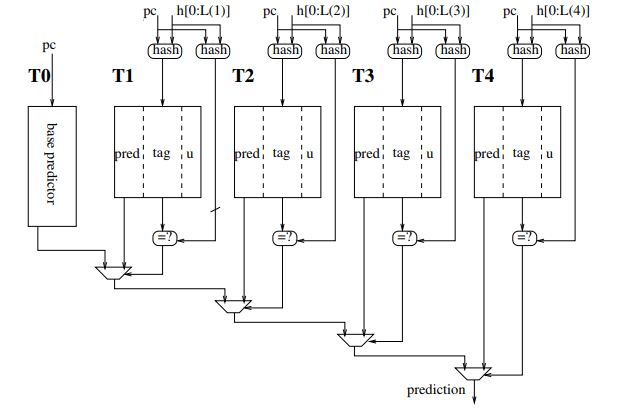
\includegraphics[width=.5\textwidth]{Imagens/ltage.PNG}
\caption{Estrutura Ltage}
\label{fig:ltage}
\end{figure}

\item[Bimode]

O preditor Bimode é um algoritmo de dois níveis que trabalha com um historico de previsão global e o endereço do desvio que indexam tabelas com contadores de dois bits \cite{lee1997bi}. Conforme o padrão do histórico global um dos preditores de direção é ativado para depois o preditor de escolha dar uma previsão final para o salto, como ilustra a Figura ~\ref{fig:bimode}.

\begin{figure}[H]
\centering
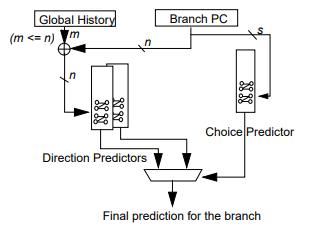
\includegraphics[width=.5\textwidth]{Imagens/bimode.PNG}
\caption{Estrutura Bimode}
\label{fig:bimode}
\end{figure}

\item[LocalBP (2bits)]

LocalBP vem de \textit{Local Branch Predictor}, um preditor de desvio que guarda um histórico local de cada desvio \cite{Patterson:1990:CAQ:77493}. O algoritmo se baseia na ideia de prever um padrão para os desvios baseado no seu historico utilizando contadores saturados de 2 bits. Cada salto possui seu contador que é alterado a cada ciclo, sendo incrementado se o salto é tomado e decrementado caso contrário como mostra a Figura ~\ref{fig:localbp}

\begin{figure}[H]
\centering
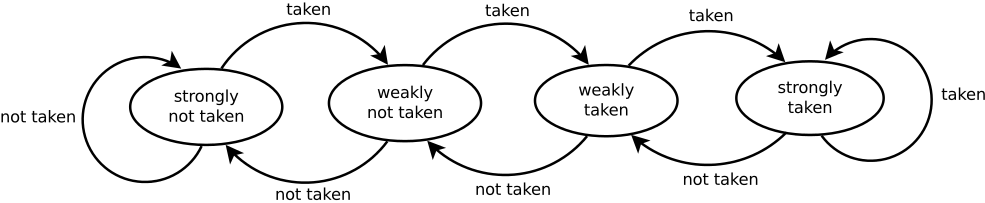
\includegraphics[width=.7\textwidth]{Imagens/contador.png}
\caption{Contador do LocalBP}
\label{fig:localbp}
\end{figure}


\item[Tournament]

O algoritmo Tournament é um híbrido de outros previsores, por si só funciona como um seletor realizando uma espécie de ``torneio" para decidir qual a melhor abordagem para cada salto \cite{Patterson:1990:CAQ:77493}. A seleção se da entre um preditor local que possui uma tabela de de histórico de saltos para cada salto, e entre um preditor global que possui uma tabela de historico global de todos os saltos processados como ilustra a Figura ~\ref{fig:tournament}. O algoritmo Tournament trabalha em cima de que existem saltos que são dependentes de informações locais enquanto outros são influenciados por informações globais.

\begin{figure}[H]
\centering
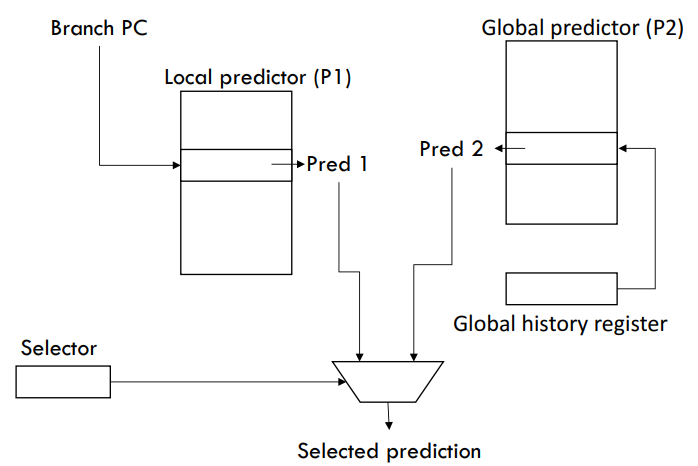
\includegraphics[width=.4\textwidth]{Imagens/tournament.PNG}
\caption{Estrutura Tournament}
\label{fig:tournament}
\end{figure}

\end{description}

\section{Avaliação}

Nesta seção será abordado a metodologia utilizada na avaliação e os resultados oriundos da mesma.

\subsection{Metodologia}

Para a avaliação dos Algoritmos de Previsão de Desvio foram feitas simulações usando o simulador Gem5.

\begin{description}

\item[Software]

Os Softwares utilizados nos experimentos foram o simulador Gem5, e os compiladores GCC e G++. Todos executados em um sistema Ubuntu 16.04.4 LTS x64.

\item[Hardware]

Os testes com o gem5 foram realizado em uma máquina em nuvem do servidor Google Cloud com as especificações: Processador Intel Xeon E5-2699, Memória RAM de 16GB e Sistema Operacional Ubuntu 16.04.4 LTS x64.


\item[Programas Utilizados]

Os preditores de desvio agiram em cima de quatro programas de entrada com diferentes propósitos como:

\begin{enumerate}

    \item \textbf{Gramschmidt} Solutor de Álgebra Linear
    \item \textbf{h264dec} Decodificador de arquivos de vídeo
    \item \textbf{Oopack\_v1p8} Comparador de desempenho entre C e C++
    \item \textbf{mandel-2} Exibe uma figura formada por astericos
    
\end{enumerate}

Para a compilação de cada programa foram utilizadas as flags -O3 para um maior nível de otimização e -static para eliminar dependências de bibliotecas dinâmicas. Somente o programa Oopack\_v1p8 foi compilado com o compilador g++, para os demais foi utiizado o gcc.

\item[Gem5]

A simulação no Gem5 foi feita em modo SE (System Call Emulation), não necessitando um sistema operacional. Com o gem5 foi construído o executável do simulador de arquitetura X86 utilizando a abordagem ``fast'' que otimiza a arquitetura ao máximo de perfomance e ignora possíveis checagens de erro.

\item[Arquitetura Simulada]

Foi modelado uma arquitetura de base para o simulador utilizando a linguagem Python com as especificações: Arquitetura X86, 2GHz de Clock, 1 Processador, CPU O3, Cache L1 separada, Cache L2 unificada e Memória DDR3\_1600\_8x8. A arquitetura foi parametrizada para receber um programa executável (binário) como entrada e um preditor de desvio.

\item[Experimentos]  

Cada um dos programas foi testado com os quatro preditores de desvios no gem5, totalizando 16 simulações. Após cada simulação foi armazenado o arquivo stats.txt com os dados da mesma como a quantidade de tentativas de predição, quantidade de predições incorretas, entre outros. Tais arquivos stats serviram como base para a avaliação de cada preditor.

\item[Avaliação]

O artigo visa analisar o melhor preditor de saltos diretos, de saltos indiretos, o que faz o melhor uso do endereço de retorno (RAS) e as diferenças no tempo de execução.

\end{description}

\subsection{Resultados}

Nesta seção será apresentado os resultados dos testes de cada programa de entrada com base nos gráficos de acerto dos desvios (Fig.~\ref{fig:adesvios}), acerto da RAS (Fig.~\ref{fig:aras}), Tempo de Execução (Fig.~\ref{fig:tempo}) e Erro de Previsão de Saltos Indiretos (Fig~\ref{fig:eindireto}). 

\begin{figure}[H]
    \centering
    \subfigure[Taxa de Acerto Previsão de Saltos Condicionais]{
        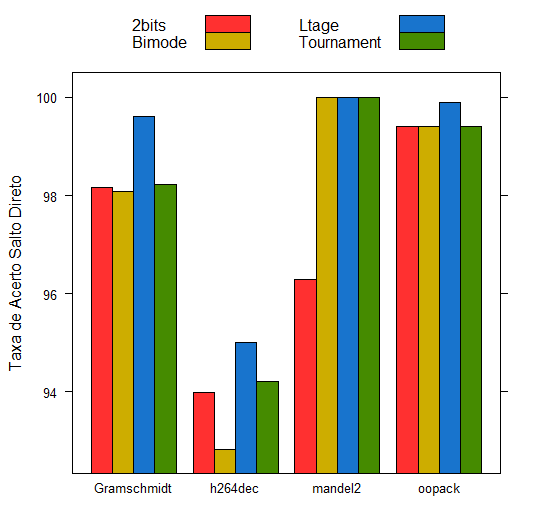
\includegraphics[width=.3\textwidth]{Imagens/acerto.png}
        \label{fig:adesvios}
    }
    \quad
    \subfigure[Erro de Previsão de Saltos Indiretos]{
        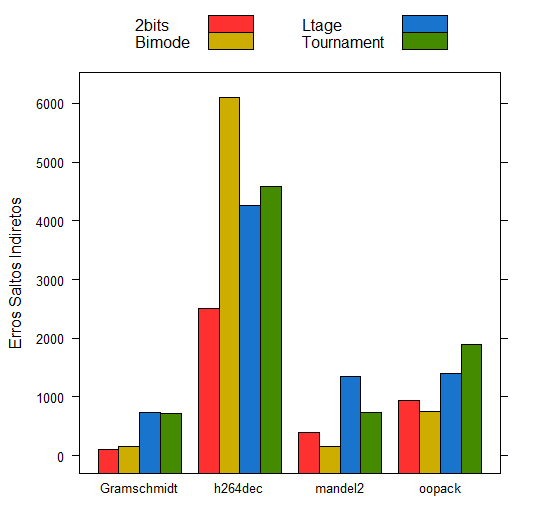
\includegraphics[width=.3\textwidth]{Imagens/erro_indireto.png}
        \label{fig:eindireto}
    }
    \caption{Previsão de Saltos}
\end{figure}

\begin{figure}[H]
    \centering
    \subfigure[Taxa Acerto RAS]{
        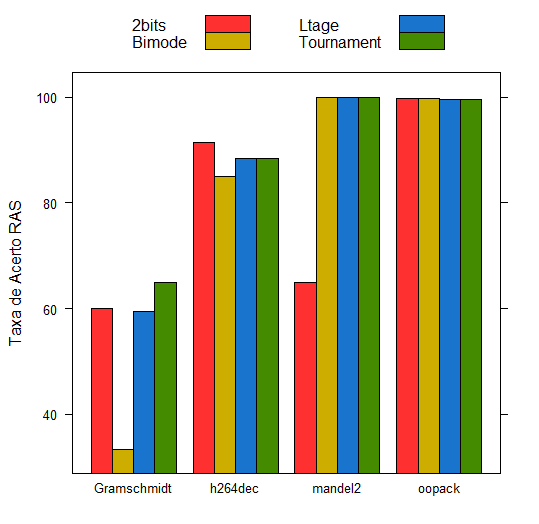
\includegraphics[width=.3\textwidth]{Imagens/acerto_ras.png}
        \label{fig:aras}
    }
    \quad
    \subfigure[Tempo de Execução]{
        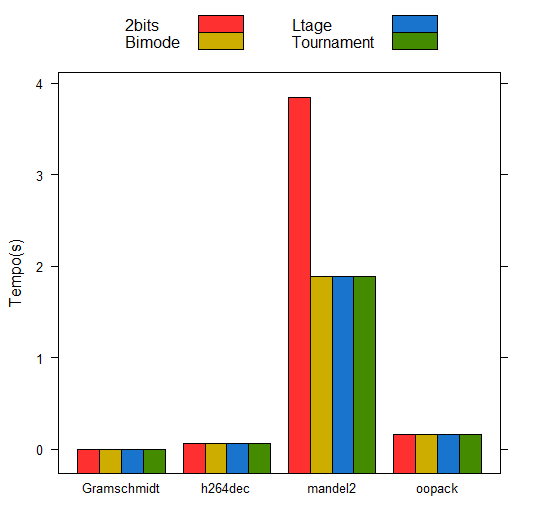
\includegraphics[width=.3\textwidth]{Imagens/tempo.png}
        \label{fig:tempo}
    }
    \caption{Previsão RAS e Tempo de Execução}
\end{figure}

\subsubsection{Previsão de Saltos Condicionais}

A taxa de acerto na previsão de saltos condidicionais teve valores proximos de 100\% para os quatro preditores, com o menor valor encontrado sendo de 92\% com o preditor Bimode no programa h264dec como ilustra a Fig.~\ref{fig:adesvios}. Dos quatro preditores o que se destaca nessa previsão é o Ltage em que nos quatro experimentos possuiu a maior taxa de acerto ou empatou com os demais como no caso do mandel-2. Seguindo o Ltage vem o Tournament que se sobressaiu ao 2bits e Bimode em metade dos casos. A análise do pior preditor de desvio é de certa forma sutil, com os preditores Bimode e 2bits tendo o pior desempenho em um experimento cada e uma taxa semelhante nos demais.

\subsubsection{Previsão de Saltos Indiretos}

Nesta previsão é possível notar um comportamento semelhante entre os preditores Ltage e Tournament que em 75\% dos casos tiveram a quantidade de erros indiretos maior que a do Bimode e 2bits. O único caso em que o Ltage e o Tournament não foram os mais custosos foi com o programa h264dec onde o Bimode os supera por uma margem considerável como mostra a Figura ~\ref{fig:eindireto}. Vale notar que o comportamento do preditor Bimode é o melhor no geral, onde somente em um caso acabou se tornando o mais custoso.

\subsubsection{Acerto RAS}

Na análise do uso do endereço de retorno na previsão foi possível notar um comportamento similar novamente entre o Ltage e o Tournament, com a mesma taxa em três testes e tendo os maiores acertos na média. Analisando a Figura ~\ref{fig:aras} pode-se afirmar que o destaque negativo vai para o Bimode que teve um desempenho inferior em metade dos casos, com um acerto menor que a metade dos outros três preditores no experimento do programa Gramschmidt. 

\subsubsection{Tempo de Execução}

O tempo de execução de cada preditor se mostrou similar com três dos quatro programas testados onde a diferença entre cada preditor não era significativa, ficando na casa dos milésimos de segundos. Como mostra a Figura ~\ref{fig:tempo} somente nos testes do programa mandel-2 o comportamento foi diferenciado, com o preditor 2bits tomando um tempo de execução duas vezes maior que os demais. Tal comportamento atípico torna difícil a afirmação a análise do tempo de execução, é possível afirmar que na média os quatro algoritmos se comportam com o mesmo tempo e que o 2bits possui um desvio maior.



\section{Conclusão}

Neste artigo foi realizada a análise de quatro Algoritmos de Previsão de Desvio, cada um com uma abordagem diferente com o objetivo de melhorar o processamento do Pipeline. Foram realizadas simulações de desempenho com o auxílio do simulador Gem5 e cinco programas diferentes de entrada. A partir das simulações foi possível montar gráficos e analisar objetivamente o desempenho de cada preditor de desvio.

A partir dos dados analisados foi possível concluir que o melhor Algoritmo de Previsão de Desvio dos analisados foi o Ltage, possuindo uma taxa de erro nitidamente menor na previsão de saltos condicionais em todos os testes. Em segundo lugar vem o Tournament que possui que embora possua um comportamento quase similar ao 2bits e o Bimode, ainda consegue se sobressair nos testes.

O contrário pode ser notado na predição de saltos indiretos onde o Ltage possui um comportamento similar ao do Tournament como os dois que possuem a maior taxa de erro, nesse quesito os destaques vão para o Bimode e 2bits, com o último possuindo o melhor desempenho.

Ainda assim, a diferença de performance do algoritmo Ltage na previsão dos desvios é significativa em todos os testes, sendo possível afirmá-lo como o Algoritmo de Previsão de Desvio de melhor desempenho dos analisados neste artigo.

\bibliographystyle{sbc}
\bibliography{Referencias.bib}

\end{document}
